\begin{evenBlock}{Secure the Box}

\begin{minipage}[t]{\linewidth}
    \centering
    
    \begin{minipage}{.3\linewidth} % Left column and width
        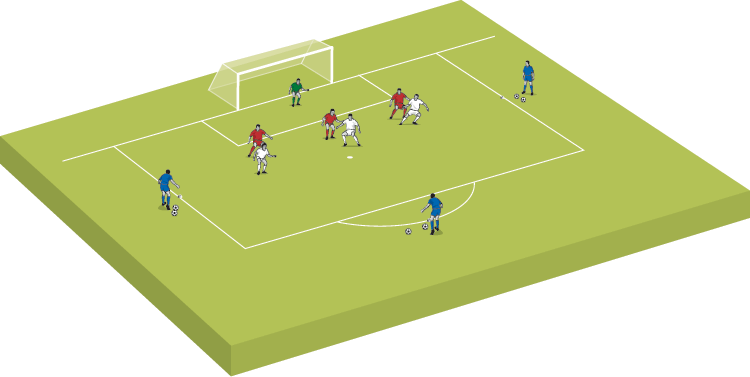
\includegraphics[width=\textwidth]{../img/Trimmed/SecureTheBox1}
    \end{minipage}
    \hspace{0.05\linewidth}
    \begin{minipage}{.6\linewidth} % Left column and width
        \textbf{Drill Description:}
        This drill is ideally played with 9 players, with 3 players per team.  With unbalanced numbers a 4th attacker could be added to create a 4v3 situation to make it harder on the defense (since this is a defensive drill).
        \begin{enumerate}
            \setlength{\itemsep}{0pt}
            \setlength{\parskip}{0pt}
            \setlength{\parsep}{0pt}
            \item The defending team must man mark, with each player picking up an attacker.
            \item The players on the edge of the area have two balls each to pass to the attackers.
            \item The serving players must pass into an attacker who is open (unmarked).
        \end{enumerate}
        
        \textbf{Coaching Points:}
        \begin{itemize}
            \setlength{\itemsep}{0pt}
            \setlength{\parskip}{0pt}
            \setlength{\parsep}{0pt}
            \item Explain marking a player is to remain within 2 or 3 feet of the attackign player.
            \item Explain how to mark a player goal side (defender between the attacker and goal).
            \item Explain how to mark a player ball side (defender between the attacker and the ball).
            \item Explain how to mark a player both goal side and ball side - defender marks the attacker goal side but is a few feet (steps) closer to the ball than the attacker.
            \item Attackers try to lose their marks.  Defenders stay marking the attacker.
            \item Defenders should communicate if they want to defend a zone or a man.  Explain to them how this can work.
            \item If zone defense is too difficult at this stage force them to play man coverage - always marking the same attacker.
        \end{itemize}

    \end{minipage}
\end{minipage}

\end{evenBlock}